\chapter{Datasets, Simulated Samples and Triggers}
\label{chap:Samples}

This analysis is based on data collected by the \ac{CMS} experiment in 2016-2018 from $pp$ collisions at a center-of-mass energy of 13 TeV corresponding to an integrated luminosity of 138 fb$^{-1}$. There were approximately 30 simultaneous $pp$ collisions occurring per 25 ns. Based on online selection criteria, fully reconstructed collision data that contain high-level physics objects are divided in ``\acp{PD}'', which include ``DoubleEG'', ``DoubleMu'', ``MuonEG'', ``SingleElectron'', and ``SingleMuon'' for 2016 and 2017 data taking era. In 2018, ``SingleElectron'', ``DoubleEG'' are replaced by ``EGamma''. The names of these \acp{PD} reflect the selection criteria. The data taking conditions in 2016-2018 were difference across the years. To account for this, all \ac{MC} samples are generated separately for each year separately. 
%%%%%%%%%%%%%%%%%%%%%%%%%%%%%%%%%%%%%%%%%%%%%%%%%%%%%%%%%%%%%
%%%%%%%%%%%%%%%%%%%%%%%%%%%%%%%%%%%%%%%%%%%%%%%%%%%%%%%%%%%%%
\section{Signal Samples}
\label{sec:Signals}

This analysis made use of signal samples that were initially produced for the LFV analysis in the dilepton channel cite{Dilepton}, which used SMEFTfr v2 UFO cite{SMEFTsim}. The datacards used to generate these samples can be found at github cite{datacards}. It was first reported by ATLAS authors cite{LHCTOP} that SMEFTfr v2 was buggy and we decided to adopt SMEFTsim v3 UFO cite{SMEFTsim} as the new CMS standard moving forward. However, it would be too late to reproduce all the samples at the time of this decision, and we decided to implement the following changes: 

The difference in kinematic distributions are shown in Fig\ref{fig:reweight}. A reweighting tool cite{reweight} is used to emulate the kinematic distributions produced by SMEFTsim. In addtion to the shape components, we updated the top production cross sections from cite{Dilepton}, which are summarized in Table ref{tab:signal}. The top decay cross sections are kept the same because they do not come from UFO.

\begin{figure}[tbh!]
 \begin{center}
 \begin{tabular}{cc}
  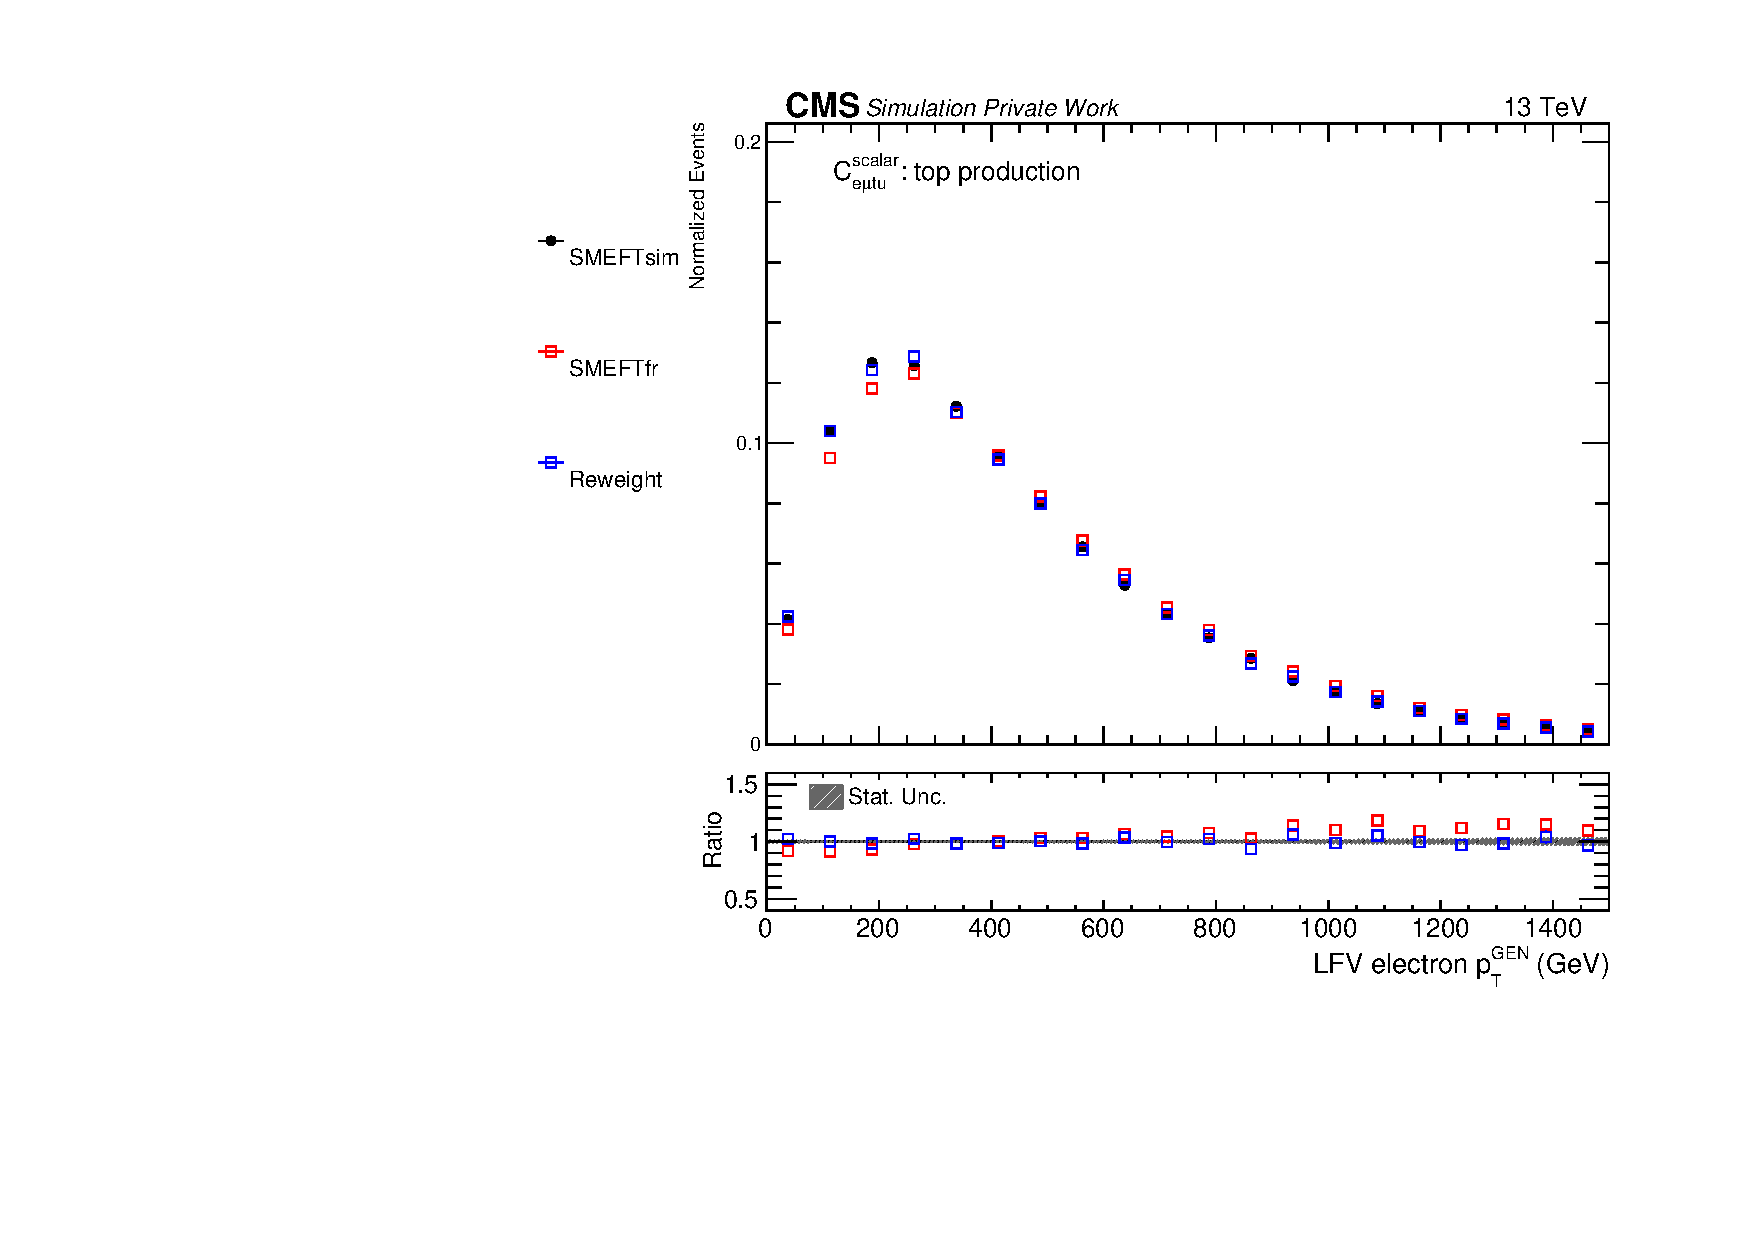
\includegraphics[width=0.48\textwidth]{figures/Part3/Samples/LFVePt}&
    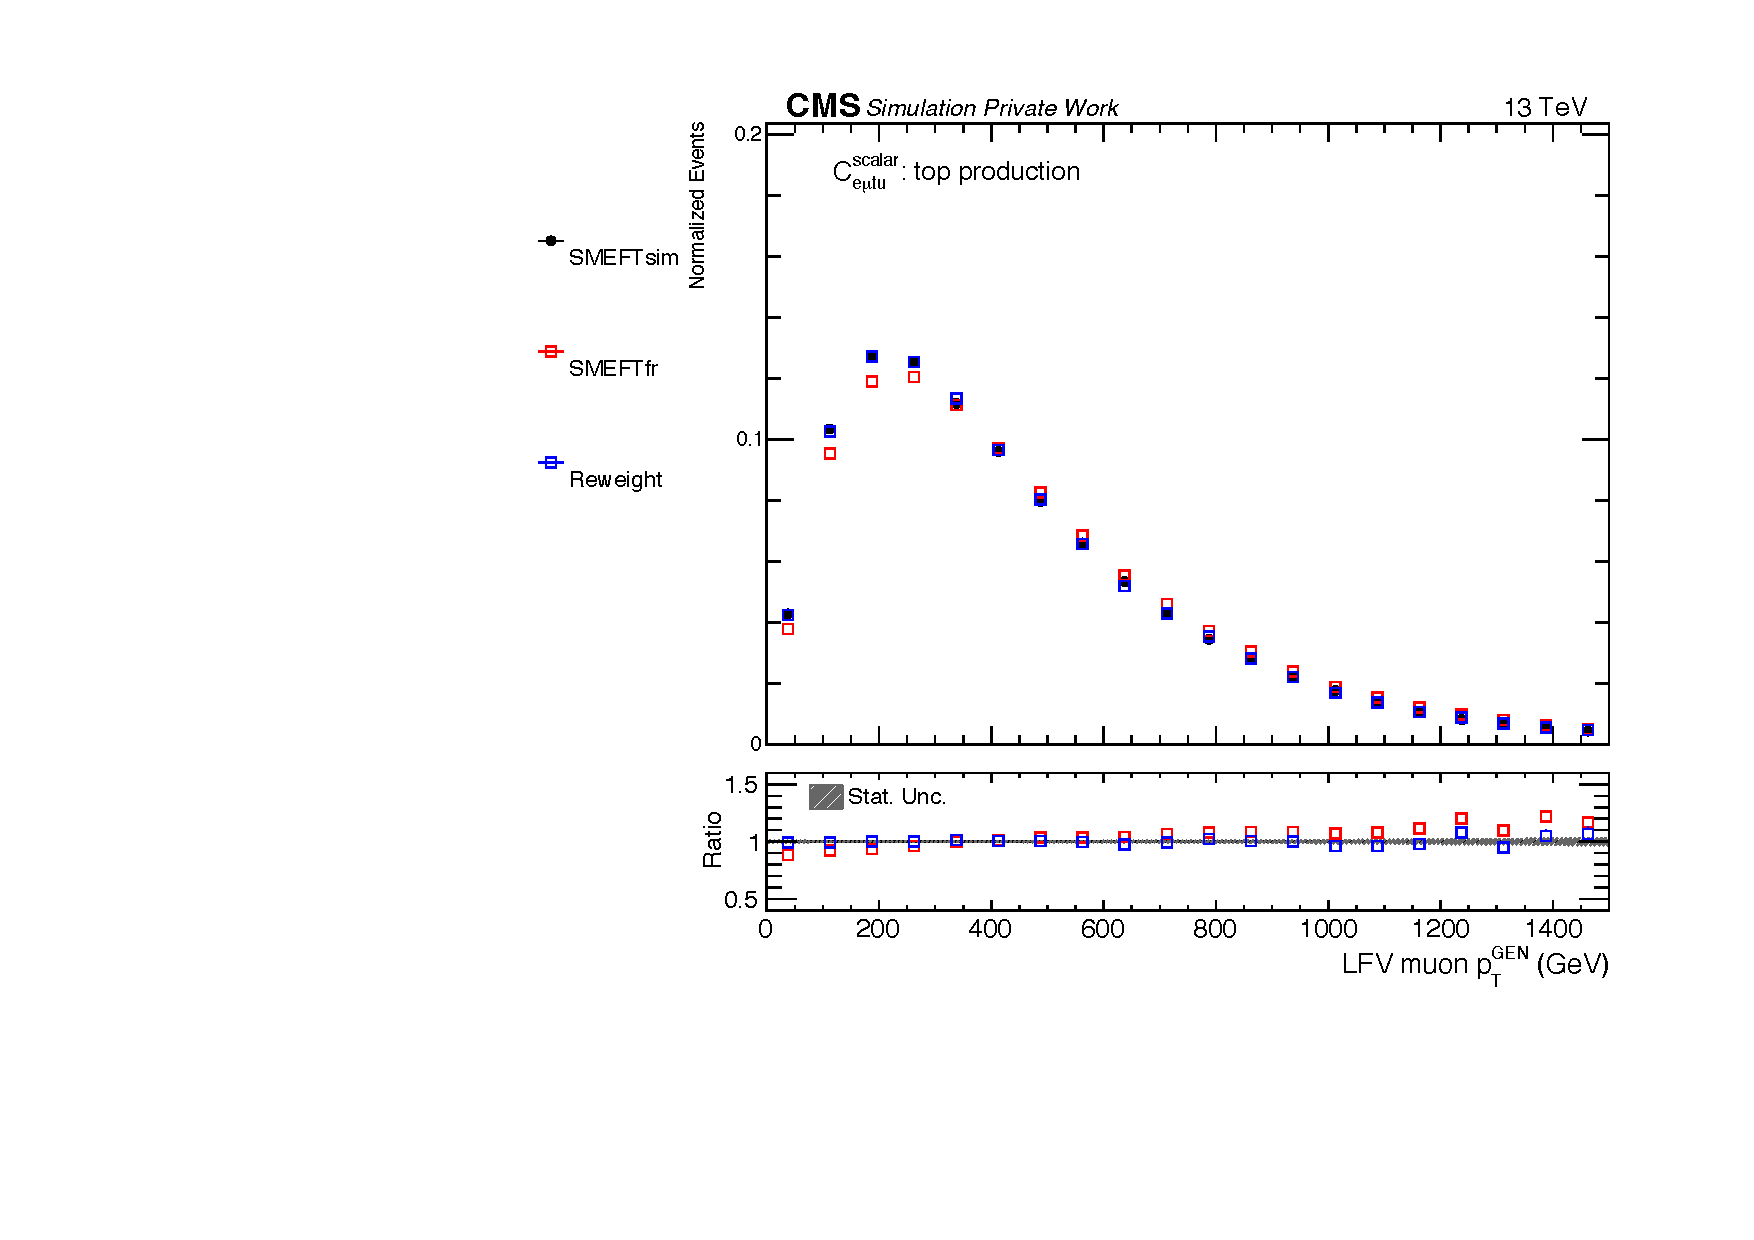
\includegraphics[width=0.48\textwidth]{figures/Part3/Samples/LFVmuPt}\\
 \end{tabular}
 \caption{Comparison of kinematic distributions produced by different UFOS: LFV electron $p_{T}$ (left), LFV muon $p_{T}$ (right). The "Reweight" (shown in blue curve) are produced by applying weights produced by cite{reweight} to EFT samples produced by SMEFTfr.}
 \label{fig:reweight}
 \end{center}
\end{figure}

\begin{table}[th]
\centering
\caption{Theoretical cross sections for top production and decay for each CLFV coupling. Uncertainties related to PDF and QCD scale are given ($\sigma^{+\text{scale}}_{-\text{scale}}\pm \text{PDF}$).}
\begin{tabular}{clll}
\toprule 
Lorentz structure    & samples              & xsection(fb)   \\  \midrule
\multirow{3}{*}{vector} & top production via u quark  & $460^{+81}_{-64}\pm6$ \\ 
      &  top production via c quark & $33^{+5}_{-4}\pm6$    \\
      & top decay via u/c quark        & $32^{+0.8}_{-1.1}\pm1.3$   \\  \midrule
\multirow{3}{*}{scalar} &top production via u quark  & $97^{+18}_{-14}\pm1$  \\ 
      & top production via c quark       & $6.3^{+0.9}_{-0.8}\pm1.4$  \\
      &  top decay via u/c quark    &  $4.0^{+0.1}_{-0.1}\pm0.2$  \\  \midrule 
\multirow{3}{*}{tensor} &  top production via u quark & $2143^{+368}_{-293}\pm31$  \\
      &  top production via c quark & $164^{+22}_{-18}\pm27$   \\
      &  top decay via u/c quark     & $187^{+5}_{-6}\pm8$   \\  \bottomrule
\end{tabular}
\vspace{-0.5em}
\label{tab:signal}
\end{table}

All but the $Q_{lq}^{(3)ijkl}$ operator in Table ref{tab:dimension6} are considered because of the equivalence of $Q_{lq}^{(3)ijkl}$ and $Q_{lq}^{(1)ijkl}$. To reduce the number of free parameters, we assume 6 independent Wilson coefficients and apply condition ref{eq1:1}-ref{eq1:6}. 

\begin{eqnarray}
\label{eq1:1}
 C_{lq}
 &=& C_{lq}^{(1)1213}
 + C_{lq}^{(1)2113}
 + C_{lq}^{(1)1231}
 + C_{lq}^{(1)1213}
 ,\\
\label{eq1:2}
 C_{lu}  
 &=& C_{lu}^{1213}
 + C_{lu}^{2113}
 + C_{lu}^{1231}
 + C_{lu}^{1213}
 ,\\ 
\label{eq1:3}
 C_{eq}
 &=& C_{eq}^{1213}
 + C_{eq}^{2113}
 + C_{eq}^{1231}
 + C_{eq}^{1213}
 ,\\
\label{eq1:4}
 C_{eu}  
 &=& C_{eu}^{1213}
 + C_{eu}^{2113}
 + C_{eu}^{1231}
 + C_{eu}^{1213}
 ,\\
\label{eq1:5}
 C_{lequ}^{(1)}  
 &=& C_{lequ}^{(1)1213}
 + C_{lequ}^{(1)2113}
 + C_{lequ}^{(1)1231}
 + C_{lequ}^{(1)1213}
  ,\\
\label{eq1:6}
 C_{lequ}^{(3)}
 &=& C_{lequ}^{(3)1213}
 + C_{lequ}^{(3)2113}
 + C_{lequ}^{(3)1231}
 + C_{lequ}^{(3)1213} 
\end{eqnarray}

The signal is simulated using MADGRAPH5$\_$aMC@NLO with SMEFT\_2l2q\_UFO\_unitary as the UFO. The signal samples are produced with an assumption that $C_a$=1, $\Lambda$=1TeV. Since all vector-like operators show similar results, we combine them and call them vector LFV signals. 
%%%%%%%%%%%%%%%%%%%%%%%%%%%%%%%%%%%%%%%%%%%%%%%%%%%%%%%%%%%%%
%%%%%%%%%%%%%%%%%%%%%%%%%%%%%%%%%%%%%%%%%%%%%%%%%%%%%%%%%%%%%
\section{Background Samples}
\label{sec:Backgrounds}

For 2016 MC, PDF set NNPDF3.0 and PYTHIA8 tune CUETP8M1 are used. In 2017 and 2018, NNPDF3.1 and PYTHIA8 tune CP5 are used. Simulated processes are divided into the following categories: $t\bar{t}$, WZ production, multi-boson production (other than WZ), the associated production of $t(\bar{t})$ and a boson or/and a quark (e.g. $t\bar{t}$W, $t\bar{t}$Z and $t\bar{t}$H) and others (e.g. W jets, DY jets). MC samples used in this analysis are summarized in Table \ref{tab:MCsample}. The cross sections of the prompt backgrounds used for this analysis are the same as the cross sections listed in cite{XSref}. The nonprompt backgrounds in this analysis will be modeled with data-driven technique. The MC samples listed in ``nonprompt" prompt category of Table \ref{tab:MCsample} are only used as reference for initial study. The charge-flip backgrounds constitute a very small contribution to the signal region.

\begin{table}
\sffamily
\caption{Summary of information related to \ac{MC} sample generation.}
\centering
 \resizebox{\linewidth}{!}{%
 \begin{tabular}{cccccc}
\toprule
 & Process & Event Generator & Perturbative QCD& Tune & XS precision \\ \midrule
\multirow{7}{*}{\vtop{\hbox{\strut Prompt}\hbox{\strut backgrounds}}}  
 &WZ&Madgraph    & NLO & CUETP8M1(CP5)   & NLO~\cite{Campbell:2011bn}    \\ 
 &ZZ &Powheg   & NLO & CUETP8M1(CP5)   & NLO~\cite{Campbell:2011bn}    \\
 &VVV &Madgraph & NLO & CUETP8M1(CP5) & NLO  \\ 
 & ttW, ttZ &Madgraph & NLO & CUETP8M1(CP5)  &  NLO~\cite{Frederix:2021agh,Kulesza:2020nfh}    \\
 &ttH & Powheg  & NLO & CUETP8M1(CP5)  & NLO~\cite{Kulesza:2020nfh}  \\ 
 &tZq &Madgraph  & NLO & CP5 & NLO    \\
 &tHq, tHW, tWZ & Madgraph    & LO & CUETP8M1(CP5)  & LO    \\
  \midrule
 \multirow{3}{*}{\vtop{\hbox{\strut Non-prompt}\hbox{\strut backgrounds}}}
 & tt & Powheg &  NLO   & CUETP8M1(CP5)    & NNLO~\cite{Czakon:2011xx}    \\ 
 & DYM50 & Madgraph   & NLO & CUETP8M1(CP5)    & NNLO~\cite{Li:2012wna}   \\
 & DYM10to50 & Madgraph   & LO  & CUETP8M1(CP5)    & NLO~\cite{Li:2012wna}    \\
  \bottomrule
  \end{tabular}}
  \label{tab:MCsample}
 \end{table} 
 %%%%%%%%%%%%%%%%%%%%%%%%%%%%%%%%%%%%%%%%%%%%%%%%%%%%%%%%%%%%%
%%%%%%%%%%%%%%%%%%%%%%%%%%%%%%%%%%%%%%%%%%%%%%%%%%%%%%%%%%%%%
\section{Triggers}
\label{sec:Triggers}

To achieve a trigger optimal acceptance, a combination of single-lepton, di-lepton and tri-lepton triggers are used to select events. These triggers are summarized in Table ref{tab:triggers16}-ref{tab:triggers18}. The following trigger logic was implemented to remove the overlap between different datasets:

\begin{itemize}
\item Events in MC datasets are required to fire at least one of the triggers listed in Table~\ref{tab:triggers16}-\ref{tab:triggers18}. 
\item Events in Single Muon datasets are required to fire at least one of the triggers listed under ``SingleMuon''. 
\item Events in Double Muon datasets are required to fire at least one of the triggers listed under ``DoubleMu''. Events are removed if they also fire at least one of the triggers listed under ``SingleMuon''.
\item Events in ``MuonEG'' datasets are required to fire at least one of the triggers listed under ``MuonEG''. Events are removed if they also fire at least one of the triggers listed under ``SingleMuon'' or ``DoubleMu''.
\item Events in Single Electron datasets are required to fire at least one of the triggers listed under ``SingleElectron''. Events are removed if they also fire at least one of the triggers listed under ``SingleMuon'' or ``DoubleMu'' or ``MuonEG''.
\item Events in DoubleEG datasets are required to fire at least one of the triggers listed under ``DoubleEG''. Events are removed if they also fire at least one of the triggers listed under ``SingleMuon'' or ``DoubleMu'' or ``MuonEG'' or ``SingleElectron''.
\item Events in EGamma datasets are required to fire at least one of the triggers listed under ``EGamma''. Events are removed if they also fire at least one of the triggers listed under ``SingleMuon'' or ``DoubleMu'' or ``MuonEG''.
\end{itemize}
